\documentclass[letterpaper, 12pt]{article}

\usepackage{graphicx}
\usepackage{longtable}
\usepackage{rotating}
\usepackage{dcolumn}
\usepackage{listings}
\usepackage{subfiles}

% Code listing commands
\lstset{language=R,
basicstyle=\scriptsize\ttfamily,
commentstyle=\ttfamily,
numbers=left,
numberstyle=\footnotesize,
stepnumber=1,
numbersep=5pt,
showspaces=false,
showstringspaces=false,
showtabs=false,
frame=single,
tabsize=2,
captionpos=b,
breaklines=true,
breakatwhitespace=false,
title=\lstname,
escapeinside={},
keywordstyle={},
morekeywords={}
}

\begin{document}
\title{ARE213 Problem Set \#1B}
\author{Peter Alstone \& Frank Proulx}
\maketitle

\section{Problem \#1}
\subsection{Part A}

\paragraph{Wrong functional form.}
In Problem Set 1A we used linear (i.e., $ y = \beta x + \epsilon$) estimators to make ``corrections'' while the true functional form of the relationships between the covariates we included in the modern were certainly not linear.  By imposing a linear function on a non-linear data generating process (described by the CEF), we introduce misspecification bias in the model.  

\paragraph{Omitted Variables Bias.}  We were able to use variables included in the dataset in our linear model, but not the unobserved variables that may be important for control.  If omitted variables exist that both determine outcomes related to birth weight and are correlated with smoking status we will over- or under-estimate the effect (depending on the characteristics of the omission).   


\subsection{Part B}

We can attempt to reduce the magnitude of the first source of bias mentioned above (functional form) by introducing non-parametric series estimators as a replacement for linear regression.  To implement this we used a natural cubic spline with two knots on the ``dmar" variable (maternal age) in the regression from PS1A.  The tobacco use (treatment) and marital status remain as factors.  We also implemented a version of the model with interactions between the splined maternal age term and the two discrete terms.  The summary of the results are in Table \ref{tab:splineresults}.  The ATE for the model we used in PS1A for tobacco use was 200 grams (rounded from an exact estimate of 195 grams).  This is essentially unchanged with the addition splines to the maternal age relationship (an exact estimate of 199 grams).  Adding interaction terms results in an ATE for tobacco use of 220 grams.  

The benefits to applying splines in this case is that the regression model more closely matches the reality of the data, which show that birth weight's relationship to maternal age has a peak and is not monotonically increasing.  The drawback is that the true functional form is only obscured in this approach.  While the interaction terms result in an ATE that is different from the one in a non-interacting model, the interpretation becomes much more difficult.  In a policymaking environment the addition of splines and interactions would represent a potential roadblock to the essential message, which remains unchanged, which is that birth weight is reduced in mothers who use tobacco (by about 200 grams).  

\let\clearpage\relax
\subfile{splineresults.tex}

\section{Problem \#2}

The Propensity Score Method (PSM) uses a ``surrogate'' normalized metric (p-score) as a replacement for the observable controls that would normally be used to condition the estimates of a treatment response to the variable in question.  The p-score is defined as a normalized score that represents the likelihood a sample selects into treatment conditioned on observables.  Because it collapses all the dimensions into a 0:1 continuum PSM avoids the curse of dimensionality encountered with large nonparametric regression models, where it can be difficult to find neighbors or ``bandwidth-mates'' in n-dimensional space.  

\subsection{Part A}

To calculate the propensity score, we estimated a logit model of mother's tobacco use (0=non-smoker, 1=smoker) as determined by the predetermined covariates shown in Table \ref{tab:propensities}. Model \#1 shows the full model using all of the covariates suspected to be predetermined. Model \#2 is a reduced form of the same model, preserving just those covariates that were significant at the 1\% level in Model \#1. 

\let\clearpage\relax
 \subfile{propensityscores.tex}

To test whether the propensity scores predicted by these two models are significantly different  we perform a likelihood ratio test between  the full and reduced model. This test yields the following output:

\paragraph{Likelihood ratio test for MLE method:} Chi-squared 3 d.f. =  10.21274, P value =  0.01684173 

The likelihood ratio test result (i.e., p $<$ 0.05 but not $<$ 0.01) indicates that the reduced-form model and full model are significantly different from each other at the 0.05 confidence level. Given this and the fact that the reduced-form model has a higher AIC, we will work with the reduced-form model of propensity scores throughout the remainder of the assignment.

\subsection{Part B}

In this section, we estimate a linear model controlling for the propensity score. This model is of the form
\begin{equation*}
dbrwt_i = \alpha + \delta_1 * tobacco_i + \delta_2 * tobacco_i * p(X_i) + \Beta * p(X_i) + u_i
\end{equation*}

The estimated coefficients for this model are given in Table \ref{tab:propensitymodel}. 

\subfile{propensityscoremodel.tex}

The estimated average treatment effect is given by 
\begin{equation}
\delta_1 + \delta_2 \overline{p}(X_i)=-237.099 + (0.1594 * 90.427)=-222.69
\end{equation}

This method assumes that treatment effects are not heterogenous with respect to $X_i$, that treatment effects \emph{are} heterogenous with respect to $p(X_i)$, and that we have unconfoundedness (i.e. the decision to smoke is randomly assigned, conditioned on exogenous variables).

Pursuant to these assumptions, the estimated ATE of smoking on birthweight based on the corrected regression method is a reduction of 223 grams.

\subsection{Part C}
We estimate the average treatment effect of smoking on birthweight to be 222 grams when using the reweighting approach. This approach involved taking a weighted average of all observations using the (normalized inverse) of the propensity score as a weighting factor. This is consistent with the estimate produced using the regression approach.

We estimate the average treatment on the treated to be 

\subsection{Part D}
Here we estimate the density function with a kernel density estimator, using the density() function in R. We estimate the density function separately for the smoking and non-smoking members of the sample, and weight their responses with the propensity scores normalized to the subsample (e.g. $p(X_i)/\sum\limits{j=1}^{N_{smokers}}p(X_j)$)

We estimate the density function using the Epanechnikov kernel and bandwidths ranging from 10 grams to 100 grams in increments of 10 grams. Figure \ref{fig:kernel40} shows the density function estimated with a bandwidth of 40 grams. This bandwidth appears to be a good compromise between washing out some of the noise at lower bandwidths while preserving the underlying CEF. 

\begin{figure}[h!]
   \centering
   \includegraphics[width=6in]{img/kerndensity40.pdf} 
   \caption{Birthweight density function estimates produced using Epanechnikov kernel estimator for smokers and non-smokers.}
   \label{fig:kernel40}
\end{figure}

We also estimate the density at $x=3000$ grams by hand. We first calculate the average propensity score for both smokers and non-smokers with infants at 3000 grams. The dataset has 12 smokers and 47 non-smokers with infants born at this weight. The average propensity score for these smokers is 0.27 and for non-smokers it is 0.20. These values stand to reason- the people who have opted in to smoking in this class have been predicted as more likely to be smokers.


\subsection{Part E}

Figure \ref{fig:kernelbw} shows how the character of the kernel density estimator is effected by the choice of bandwidth for the problem at hand.  While all the kernel densities tend to tell the same story, those with ``middle" bandwidth are a good balance between the choppy nature of small bandwidth and over-smoothing of large bandwidth.

\begin{figure}[h!]
   \centering
   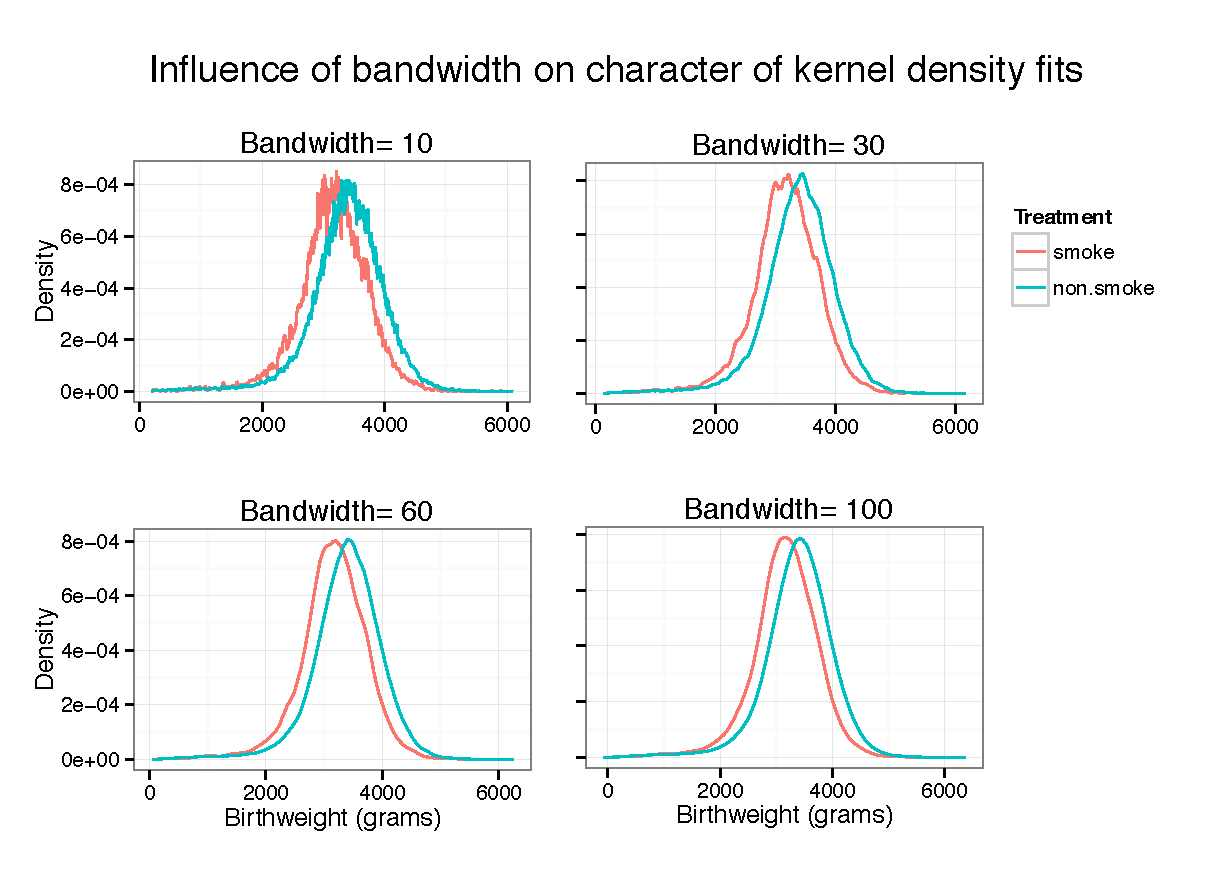
\includegraphics[width=6in]{img/kdens-combinebw.pdf} 
   \caption{Comparison of bandwidth choices for birthweight density function estimates produced using Epanechnikov kernel estimator for smokers and non-smokers.}
   \label{fig:kernelbw}
\end{figure}

\subsection{Part F}

The weighting approach in Part C offers a way to use propensity scores in a regression model, so it is possible to ``tell a story" with the results that is accessible to people who are comfortable with regression models.  TODO: Add text here. 

The potential downside to the weighting scheme is that outliEr values (very high or low propensity scores) for those who went ``against" their propensity (i.e., for a low score, they selected to treatment or vice versa) will have very high weight (approaching infinity in the limit).  It is possible to mitigate this issue by trimming the data to only consider people with propensity scores between 10 \% and 90\%, for instance.  

\subsection{Part G}
Using a range of propensity scoring methods we find that the average effect of smoking on birth weight is 220 grams (lower weight for mothers who smoke).  Both regression adjustment and reweighing methods resulted in essentially the same result, which matches the result of using cubic splines and interaction in a regression model.  

TODO: Finish writing interpretation.
\section{Problem \# 3}
Here we use a blocking approach to estimate the Average Treatment Effect. This entails subdividing all of the observations into evenly spaced blocks based on propensity scores. The average treatment effect is estimated within each blocks by calculating the average birthweights of children to smokers and to non-smokers separately and taking the difference. Any blocks with 0 smokers or 0 non-smokers are discarded, as no ``match'' has been made here. Finally, the average treatment across blocks is taken, weighting each block based on the number of observations within the block. 
The block sizes produced using this method are displayed in Figure \ref{fig:blocks}. In this plot, the histograms are plotted on top of each other to demonstrate how the smokers and non-smokers are distributed with respect to each other.

\begin{figure}[h!]
   \centering
   \includegraphics[width=6in]{img/blockplot.pdf} 
   \caption{Overlaid plot of block group sizes, before cleaning.}
   \label{fig:blocks}
\end{figure}

The Average Treatment Effect estimated using the blocking method is 217 grams. This is again very close to the other values that we have estimated.

\section{Problem \#4}
Because low birth weights (<2500 grams) are of particular concern, we again use the blocking method to estimate the Average Treatment Effect of smoking on the probability of having a low birth weight. The steps taken are very similar to those taken in Problem \#3. However, now we have calculated an indicator variable for every observation in the dataset corresponding to low birth weights. Within each block, we take the proportion of smokers and non-smokers who have given birth to low birth weight infants as the probability of this occuring. The within block treatment effect is thus the difference in probability of the low birth-weight event occuring. Using this method, we estimate an Average Treatment Effect of smoking on low birthweight of 3.78\%, which is to say that smokers are 3.78\% more likely than non-smokers to produce babies in the low birth weight range.

\section{Problem \#5}
In this assignment, we have estimated the Average Treatment Effect of tobacco use by mothers on infant birthweights using a variety of methods. 

\section{Code}
We used R to complete this assignment.  The code is below:

\lstinputlisting{ps1b.R}
\lstinputlisting{../util/are213-func.R}

\newpage
\thispagestyle{empty}
\mbox{}

\end{document}
